% =====================================================================
% NegoPlay — FINAL PROJECT PORTFOLIO — PhD-LEVEL EDITION
% This is the doctoral-grade revision of final_portfolio.tex. It keeps the
% experimental results unchanged but upgrades terminology, formalises the
% methodology mathematically, anchors every stage in the peer-reviewed
% literature, and adds a generative-AI disclosure + publication roadmap, per
% the academic-review recommendations (June 2026).
% Build: xelatex final_portfolio_phd.tex (twice)
% =====================================================================
\documentclass[11pt, a4paper, oneside, openany]{report}

\usepackage[a4paper, margin=2.4cm]{geometry}
\usepackage{graphicx}
\usepackage{pdfpages}
\usepackage{booktabs}
\usepackage{tabularx}
\usepackage{enumitem}
\usepackage{float}
\usepackage{xcolor}
\usepackage{listings}
\usepackage{titlesec}
\usepackage{amsmath}
\usepackage{amssymb}
\usepackage[hidelinks]{hyperref}

\definecolor{navy}{HTML}{16324F}
\definecolor{steel}{HTML}{2C5F8A}
\definecolor{codebg}{HTML}{F4F6F8}

\titleformat{\chapter}[hang]{\bfseries\LARGE\color{navy}}{\thechapter\quad}{0pt}{}
\titlespacing*{\chapter}{0pt}{-20pt}{18pt}
\titleformat{\section}{\bfseries\Large\color{steel}}{\thesection\quad}{0pt}{}

\lstset{
  basicstyle=\ttfamily\footnotesize,
  backgroundcolor=\color{codebg},
  frame=single, framerule=0.3pt, rulecolor=\color{steel!40},
  breaklines=true, columns=fullflexible,
  keywordstyle=\bfseries\color{navy},
  commentstyle=\itshape\color{gray},
  language=Python, showstringspaces=false,
  xleftmargin=6pt, xrightmargin=6pt, aboveskip=8pt, belowskip=8pt
}

\begin{document}

% =====================================================================
% PAGE 1 — TITLE PAGE
% =====================================================================
\begin{titlepage}
\centering
\vspace*{1.8cm}
{\color{navy}\rule{\textwidth}{1.2pt}}\\[1.2cm]
{\Huge\bfseries\color{navy} NegoPlay\\[0.45cm]}
{\Large From Bridge Tables to the Negotiation Table:\\
Do Decision-Making Styles Transfer Across Domains?\\[0.6cm]}
{\normalsize\itshape An empirical study of cross-domain behavioural
consistency in game-derived LLM agents\\[1.0cm]}
{\color{navy}\rule{0.6\textwidth}{0.6pt}}\\[1.4cm]
{\large \textbf{Final Project Portfolio}\\
Final Summary Report \,\textperiodcentered\, Preparatory Report \,\textperiodcentered\, Business Plan\\[1.8cm]}
\begin{tabular}{rl}
\textbf{Submitted by:} & Anna Ben-Shushan \\[6pt]
\textbf{Course lecturer:} & Dr.\ Yoram Segal \\[6pt]
\textbf{PhD supervisor:} & Dr.\ Nezer Jacob Zaidenberg \\[6pt]
\textbf{Course:} & AI Development Expert \\[6pt]
\textbf{Institution:} & TESI - The External Studies Institute \\[6pt]
\textbf{Version:} & 9.0 \\[6pt]
\textbf{Submission date:} & June 14, 2026 \\
\end{tabular}\\[1.1cm]
{\small Code \& data:\ \href{https://github.com/annafr2/From-Bridge-Tables-to-Global-Markets}{\color{steel}github.com/annafr2/From-Bridge-Tables-to-Global-Markets}}\\[1.1cm]
{\color{navy}\rule{\textwidth}{1.2pt}}
\vfill
\end{titlepage}

% =====================================================================
% PAGE 2 — EXECUTIVE ABSTRACT (~200 words, deliberately plain-language)
% =====================================================================
\chapter*{Executive Abstract}
\addcontentsline{toc}{chapter}{Executive Abstract}

Negotiation is one of the most valuable skills in business, yet it is
very hard to study: real negotiations are private, their outcomes are
rarely recorded in any standard way, and no public dataset links how a person
makes decisions to how they negotiate. \textbf{NegoPlay} addresses this gap by
using competitive bridge -- a card game in which every decision under
uncertainty is recorded and scored -- as a measurable laboratory for strategic
decision-making.

From 149{,}208 tournament records, the project identifies five distinct
decision-making styles among elite players, ranging from cautious to highly
aggressive. Each style is then turned into an AI agent that negotiates
simulated business deals, letting us ask a single question: does a player's
style carry over from the card table to the negotiating table?

It does. \textbf{Style transfers strongly} -- aggressive bridge players
negotiate aggressively, and cautious players negotiate cautiously (a rank
correlation of about $0.80$, where $1.0$ is perfect agreement) -- whereas the
ability to \emph{win} transfers far less cleanly, because winning also depends
on the opponent. A control experiment, in which the styles are deliberately
swapped, confirms that the carry-over comes from the players' real
decision patterns rather than from how the agents were labelled.

NegoPlay offers early, reproducible evidence that decision-making
\emph{style} is a transferable trait across very different strategic domains.

% =====================================================================
% PAGE 3 — ACKNOWLEDGMENTS
% =====================================================================
\clearpage
\chapter*{Acknowledgments}
\addcontentsline{toc}{chapter}{Acknowledgments}

\vspace{0.5cm}
I would like to thank the people who accompanied this project from idea to
working system.

\vspace{0.4cm}
\textbf{Dr.\ Yoram Segal}, for the engineering-first project framework that
shaped this work (the single-SDK discipline, the insistence on measurable
deliverables, and the standard that a research prototype should still be a
well-built piece of software) and for sharp methodological guidance: the
demand for baselines, preprocessing audits, and statistical honesty pushed
this project to validate every number it reports, including the
random-baseline test that reshaped the bridge metric.

\vspace{0.3cm}
\textbf{Prof.\ Jari H\"am\"al\"ainen} (LUT University), my PhD supervisor,
for the academic home in which this project serves as the empirical baseline.

\vspace{0.3cm}
\textbf{Dr.\ Nezer Jacob Zaidenberg}, for bridge-domain expertise: from
sample-size corrections in profile discovery to the double-dummy reference
that anchored the skill metric.

\vspace{0.3cm}
And finally, my family, for their patience with me throughout this journey:
for the many hours I was absent, immersed in studies and in building this
project. Thank you for the understanding and support that made it possible.

% =====================================================================
% USE OF GENERATIVE AI (LUT disclosure requirement)
% =====================================================================
\clearpage
\chapter*{Use of Generative AI}
\addcontentsline{toc}{chapter}{Use of Generative AI}

In accordance with LUT University's guidelines on the use of generative
artificial intelligence in research and theses (effective 1 June 2024), the
author discloses the following.

\vspace{0.3cm}
\textbf{As an object of study (methodology).} Large language models are the
main subject of this project. Google Gemini (Flash~2.x) is the default
provider for the NegoPlay agents, with Anthropic Claude and OpenAI available
for cross-provider validation. This use is an integral, documented part of the
experimental design (Chapter~\ref{ch:ai}) -- it is the system under
investigation, not a writing aid.

\vspace{0.3cm}
\textbf{As a writing and engineering assistant.} Generative AI tools
(Google Gemini and Anthropic Claude) were additionally used to assist with
language polishing, proofreading, improving semantic transitions, refining the
academic style of the English text, and as a coding assistant for software
implementation and document typesetting.

\vspace{0.3cm}
\textbf{Author's declaration.} All scientific content of this work --
the research questions, the experimental design, the empirical analyses, the
algorithms, the interpretation of results, and the conclusions -- is the
author's own independent work. Generative AI was not used to produce original
research findings or scientific claims.

% =====================================================================
% TABLE OF CONTENTS
% =====================================================================
% Make an EMPTY \numberline{} (used by the bundled sub-reports, whose TOC
% entries carry no master chapter number) collapse to zero width, so their
% titles sit flush-left at the same margin as Part I's numbered chapters
% instead of being indented by a reserved-but-blank number box. Numbered
% entries (Part I) keep the original behaviour untouched.
\makeatletter
\let\nl@orig\numberline
\renewcommand{\numberline}[1]{\def\nl@tmp{#1}\ifx\nl@tmp\@empty\else\nl@orig{#1}\fi}
\makeatother
\clearpage
\tableofcontents
\clearpage

% =====================================================================
% PART I — FINAL SUMMARY REPORT
% =====================================================================
\part{Final Summary Report}

\chapter{Project Overview}

\section{The problem and the idea}
Business negotiation is one of the most important skills in industry, yet
it is nearly impossible to study quantitatively: transcripts are confidential,
outcomes are not standardised, and no public dataset links a person's
decision style to their negotiation behaviour. Competitive bridge offers a
way around this. Every deal is a sequence of recorded decisions under
uncertainty - how high to commit, when to take a risk, when to fight -
and every decision has a measurable outcome. NegoPlay treats bridge as a
\emph{behavioural laboratory}: discover decision-making profiles in bridge
data, embody them in LLM agents, and test whether the style they encode
transfers to a different strategic domain. Methodologically this mirrors the
testbed logic of modern game AI \cite{silver2017} -- a structured game is used
to study a general capability -- and it builds on a line of work that learns
explicit behavioural profiles from gameplay telemetry \cite{talwadker2022} and
treats unknown counterparts as mixtures of a few cardinal strategy types
\cite{lockett2007}.

\section{System pipeline}
The system is a four-stage hybrid pipeline (classical ML $\rightarrow$ LLM),
connected by persisted file artefacts:

\begin{enumerate}[leftmargin=*]
  \item \textbf{Profile discovery (ML).} 149{,}208 EuroBridge records
        $\rightarrow$ 8 behavioural features per player. We first ran the
        standard unsupervised pipeline (scikit-learn
        \texttt{StandardScaler} $\rightarrow$ \texttt{PCA} $\rightarrow$
        K-Means, cross-checked with HDBSCAN and a Gaussian mixture),
        but the silhouette score never exceeded $0.15$: elite players form
        a smooth \emph{continuum}, not separable blobs. This is a real
        finding, not a clustering failure (Chapter~\ref{ch:formal}): we
        therefore treat the five profiles as behavioural \emph{archetypes} --
        the extreme points of that continuum -- and assign them by
        \textbf{extreme-percentile thresholding} (top $P\%$ on a profile's
        defining axis) gated by a one-sided binomial significance test
        ($p<0.05$ versus the population baseline,
        \texttt{scipy.stats.\allowbreak binomtest}) $\rightarrow$ 5 profiles:
        four behavioural archetypes (Slam Hunter, Insurance Player, Fighter,
        NT Specialist) plus a Generalist baseline -- the population centroid
        the archetypes are measured against. All five ($K=5$) are carried into
        the cross-domain analysis.
  \item \textbf{Skill extraction (LLM).} Real hands per profile are chunked
        and sent to the LLM, which returns 5--7 characteristic skills as
        structured JSON.
  \item \textbf{Agent construction.} Each profile becomes an agent whose
        character card contains \emph{only} the bridge-derived skills -
        never personality adjectives (the anti-tautology rule, formalised in
        Chapter~\ref{ch:formal} as an \emph{identity-disentangled crossover
        control}).
  \item \textbf{Dual simulation and alignment.} The agents bid bridge deals
        and negotiate business scenarios; behaviour and outcomes in the two
        domains are correlated.
\end{enumerate}

\section{Data}
\begin{itemize}[leftmargin=*]
  \item \textbf{Bridge:} 149{,}208 board records from the public EuroBridge
        championship database (2016--2025), scraped with a custom Python
        pipeline; 563 players pass the $\geq 50$-board reliability threshold.
  \item \textbf{Negotiation (external validation):} 5{,}247 real human
        price negotiations (Stanford Craigslist Bargains corpus
        \cite{he2018}), used to validate the behavioural features and to
        calibrate the simulated seller.
\end{itemize}

% =====================================================================
% NEW CHAPTER — FORMAL FRAMEWORK AND POSITIONING
% =====================================================================
\chapter{Formal Framework and Positioning in the Literature}
\label{ch:formal}

This chapter states the project's claims in formal terms and anchors each stage
of the pipeline in the peer-reviewed literature, so that the empirical results
of Chapter~\ref{ch:keyresults} can be read against established methodology.

\section{From ``style transfer'' to cross-domain behavioural consistency}
The phenomenon this project measures is best named
\textbf{cross-domain behavioural consistency} (CDBC): the degree to which the decision
dispositions a player exhibits under uncertainty -- represented as a strategic
policy -- are preserved when the agent is moved to a semantically different
environment.\footnote{We avoid the bare term \emph{style transfer}.
In machine learning that phrase denotes a specific family of
convolutional-network techniques for recombining the artistic style and visual
content of images; it does not describe the transfer of a decision-making
policy between strategic environments.} The colloquial phrasing ``style
transfers'' is retained only as an intuition.

The premise that an LLM can internalise an abstract strategic disposition from
structured interaction and apply it in a different setting is supported by
recent work: Tennant et al.\ \cite{tennant2025} show that LLM agents
acquire stable cooperative-versus-self-interested dispositions from
game-theoretic play and exhibit them across game types. Their mechanism is
reward-based fine-tuning, whereas NegoPlay induces the disposition purely at
the prompt level through bridge-derived skills, with no fine-tuning -- a
simpler route to the same kind of cross-context consistency.

\section{Profiles as behavioural archetypes}
The low silhouette score is itself a result: elite players do not fall into
disjoint clusters but populate a smooth behavioural continuum.
The appropriate framing is therefore \textbf{archetypal boundary profiling}:
rather than partitioning the population, we identify the extreme points
(archetypes) of the behavioural space, of which every real player is
effectively a blend. This is the logic of archetypal analysis
\cite{cutler1994}, in which observations are expressed as convex combinations
of a few extremal archetypes, and it parallels the practice of modelling an
unknown opponent as a mixture over a small set of \emph{cardinal} strategies
\cite{lockett2007}. The five NegoPlay profiles are exactly such a cardinal set:
a low-dimensional basis with which any counterpart's decision profile can be
described. The unsupervised discovery of behavioural profiles from raw gameplay
records also follows established practice in skill-gaming analytics
\cite{talwadker2022}.

Sampling the \emph{tails} of the behavioural distribution rather than its
dense centre is a deliberate design choice, not merely a small sample. The
archetypes are the most behaviourally distinct players, so concentrating on
them maximises the stylistic signal available for the cross-domain test; the
price is statistical power, which is reported honestly as a limitation
(Chapter~\ref{ch:keyresults}). Establishing the effect on these representative
extremes first, then widening to the continuum, is the natural order for a
proof of concept.

\section{The zero-intelligence baseline}
A skill metric is only meaningful if a non-strategic agent scores poorly under
it. We therefore include a \textbf{zero-intelligence agent with constraints}
(ZI-C) -- informally, a ``random monkey'' bidder -- which selects uniformly at
random from the set of \emph{legal} actions in each state. This is the
classical zero-intelligence construction of Gode and Sunder
\cite{godesunder1993}, whose central result is that much of the apparent
efficiency of a market (or, here, of a scoring proxy) can be an artefact of the
constraints rather than of intelligent play. The ZI-C agent thus establishes a
clear lower bound that separates the influence of the game's rules from
genuine skill.

\section{Identity-disentangled crossover control}
The cardinal engineering rule -- that agents are described only by extracted
bridge skills, never by personality labels -- is enforced and tested by an
\textbf{identity-disentangled crossover control}. Each profile retains its
semantic identity label but is given the operative decision rules (skills) of
the \emph{opposite} profile. Because the behavioural outcome follows the
injected skills rather than the label (Chapter~\ref{ch:keyresults}), this
disentangles the effect of the operative policy from any attribution bias of
the language model, ruling out the tautology ``the agent is aggressive because
we called it aggressive.''

\section{Modelling the negotiation domain}
The negotiation side follows the standard separation of strategic intent from
surface language in negotiation dialogue systems \cite{he2018}: the agent first
decides a coarse act (counter / accept / walk away) and a target price, and the
seller is an objective, fixed counterpart calibrated on the same Craigslist
Bargains corpus \cite{he2018}. This keeps the measured quantity -- how
aggressively each profile opens -- a property of the agent's disposition, not
of a variable opponent.

% =====================================================================
% NEW CHAPTER — MATHEMATICAL FORMULATION
% =====================================================================
\chapter{Mathematical Formulation}
\label{ch:math}

This chapter gives the formal definition of each pipeline stage. All constants
below are the values actually used in the implementation.

\section{Feature standardisation and variance filtering}
Let $X \in \mathbb{R}^{n \times p}$ be the raw feature matrix, where
$n = 563$ is the number of players passing the reliability threshold
($\geq 50$ declared boards). For player $i$ and feature $j$, the standardised
score is
\begin{equation}
z_{ij} = \frac{x_{ij} - \mu_j}{\sigma_j},
\qquad
\mu_j = \frac{1}{n}\sum_{i=1}^{n} x_{ij},
\qquad
\sigma_j = \sqrt{\frac{1}{n}\sum_{i=1}^{n}\left(x_{ij}-\mu_j\right)^2}.
\end{equation}
Features whose coefficient of variation falls below a fixed threshold are
removed, as they carry no discriminative signal:
\begin{equation}
\mathrm{CV}_j = \frac{\sigma_j}{\lvert \mu_j \rvert} \;\geq\; 0.10 .
\end{equation}
In the empirical data this rule dropped \texttt{avg\_level}
($\mathrm{CV}=0.04$ -- almost everyone bids near level $3$) and
\texttt{avg\_bids\_per\_board} ($\mathrm{CV}=0.08$), leaving the
discriminative behavioural features.

\section{Archetype assignment via a one-sided binomial test}
A player $i$ is assigned to the archetype defined by axis $j$ only if two
conditions hold: the player lies in the top decile of that axis
($z_{ij} \geq z_{\text{thr}}$, with the extreme fraction set to the top
$10\%$), \emph{and} the behaviour is unlikely under chance. Let $n_i$ be the
player's operative denominator (e.g.\ declared boards) and $k_i$ the count of
the defining event (e.g.\ slam attempts for the Slam Hunter). Under the null
hypothesis that the player acts at the population base rate $p_0$, the
one-sided $p$-value is
\begin{equation}
p\text{-value}_i \;=\; \sum_{m=k_i}^{n_i}\binom{n_i}{m}\,p_0^{\,m}\,(1-p_0)^{\,n_i-m},
\qquad\text{assign iff } p\text{-value}_i < 0.05 .
\end{equation}
This is the sample-size guard recommended by the domain expert: a player with,
e.g., a $20\%$ slam rate over only $20$ boards is rejected as small-sample.

\section{The zero-intelligence policy}
Let $A_{\text{legal}}(s)$ be the set of legal calls in auction state $s$, as
defined by the laws of duplicate bridge. The ZI-C baseline policy draws
uniformly from the legal actions only:
\begin{equation}
\pi_{\text{ZI-C}}(a \mid s) =
\begin{cases}
\dfrac{1}{\lvert A_{\text{legal}}(s)\rvert} & a \in A_{\text{legal}}(s),\\[1.2ex]
0 & a \notin A_{\text{legal}}(s).
\end{cases}
\end{equation}

\section{Cross-domain metrics and rank correlation}
\textbf{Bridge skill.} In duplicate bridge a deal is played at two tables, so a
pair's raw score $S_k(b)$ on board $b$ is compared against the field datum
$D(b)$ (the mean score of everyone holding the same cards) and converted to
international match points through the standard non-linear map $f_{\text{IMP}}$:
\begin{equation}
\mathrm{IMP}_k(b) = f_{\text{IMP}}\!\left(S_k(b) - D(b)\right).
\end{equation}

\textbf{Negotiation aggression.} For a buyer agent $k$ facing a seller that
opens at $P_{\text{ask}}$ with reservation price (floor) $P_{\text{floor}}$,
let $P_{\text{open}}$ be the agent's first counter-offer. The demand depth is
\begin{equation}
\theta_k = \frac{P_{\text{ask}} - P_{\text{open}}}{P_{\text{ask}} - P_{\text{floor}}},
\end{equation}
i.e.\ how far down the seller's full concession range the agent opens.

\textbf{Cross-domain consistency.} With $K=5$ profiles, this consistency
is the Spearman rank correlation between the bridge-aggression
ranking (a weighted composite of slam, penalty-double, and pre-empt rates) and
the negotiation demand-depth ranking:
\begin{equation}
\rho_s = 1 - \frac{6\sum_{k=1}^{K} d_k^2}{K\,(K^2-1)},
\end{equation}
where $d_k$ is the difference in $k$'s rank between the two domains. The
measured value is $\rho_s = +0.80$; the identity-disentangled control inverts
it to $\rho_s = -0.90$ (Chapter~\ref{ch:keyresults}).

\chapter{Key Results}
\label{ch:keyresults}

\section{A trustworthy bridge metric (ZI-C baseline + double-dummy)}
A skill metric must rank a non-strategic agent last. Our first, coarse bridge
proxy (a \emph{par-proxy}: it scored a bid by how close its contract level sat
to a heuristic ``par'' derived from the partnership's high-card points,
rewarding sensible-looking aggression but never checking whether the contract
would actually succeed) failed this test: the zero-intelligence (ZI-C, random
``monkey'') bidder \emph{outscored} every expert profile (0.54 vs.\
0.25--0.51), because random bids still land near the heuristic par often
enough. Re-scoring each contract by whether it \emph{actually makes} under
double-dummy (perfect-play) evaluation of the real 52 cards collapses the ZI-C
agent to last place (0.10):

\begin{figure}[H]
\centering
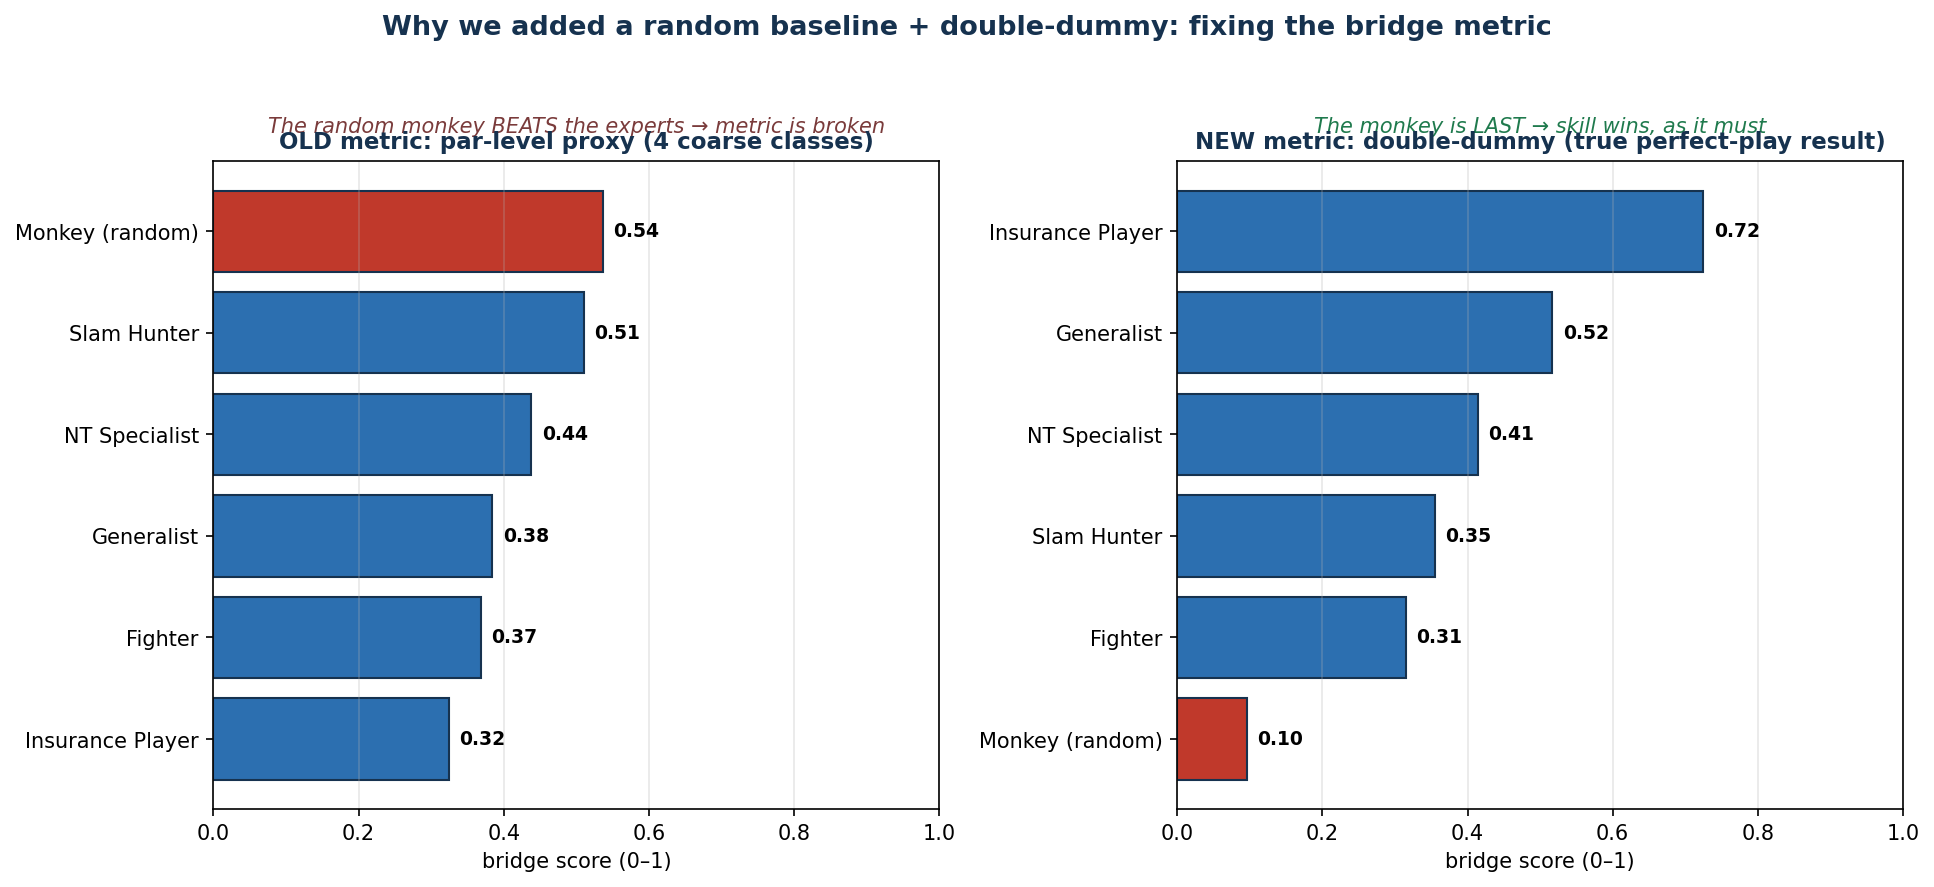
\includegraphics[width=\textwidth]{../docs/images/metric_fix_monkey_dd.png}
\caption{The zero-intelligence (ZI-C) baseline exposes (left) and the
double-dummy metric fixes (right) the bridge score.}
\end{figure}

Bridge skill was then measured from the \emph{real} competitive results.
In duplicate bridge the same deal is played at two tables, so a pair's result
can be compared against everyone else who held the identical cards: the
average raw score across the field is the \emph{datum}, and the difference is
converted to IMPs (the standard non-linear bridge scale). This is a like-for-like
skill measure (defence is captured automatically, since a poor defender simply
concedes IMPs to the field). On this scale the ZI-C agent sits at
$-7$~IMP per board (it loses heavily to the real players who held its cards),
the elite profiles cluster near $0$ (they roughly match the field, as expected
for top players), and double-dummy perfect play marks the ceiling at $+1.1$:

\begin{figure}[H]
\centering
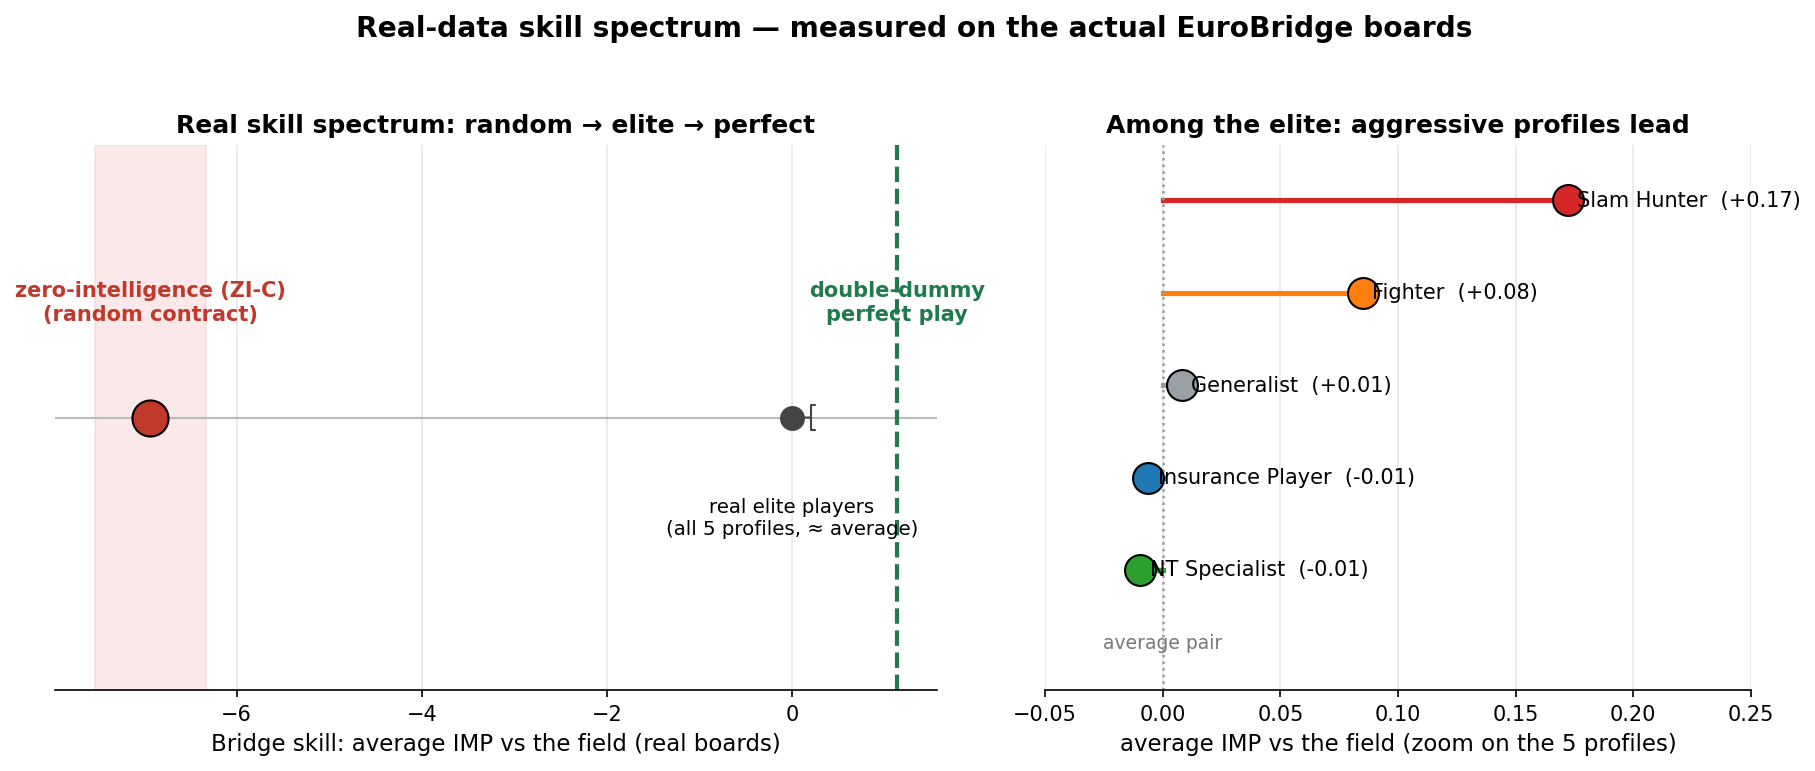
\includegraphics[width=\textwidth]{../docs/images/real_skill_spectrum.png}
\caption{Real-data skill spectrum: zero-intelligence floor $\rightarrow$ elite
players $\rightarrow$ perfect-play ceiling.}
\end{figure}

\section{The discovery: style transfers, winning does not}
Correlating \emph{winning} across domains proved weak and metric-sensitive
($\rho \approx +0.2$ to $+0.5$), because whether a style wins depends on the
opponent and the payoff rules. Refining the question to its original
behavioural form - does an aggressive bridge profile \emph{bargain}
aggressively? - yields cross-domain behavioural consistency of
\textbf{Spearman $\rho = +0.80$}:

\begin{figure}[H]
\centering
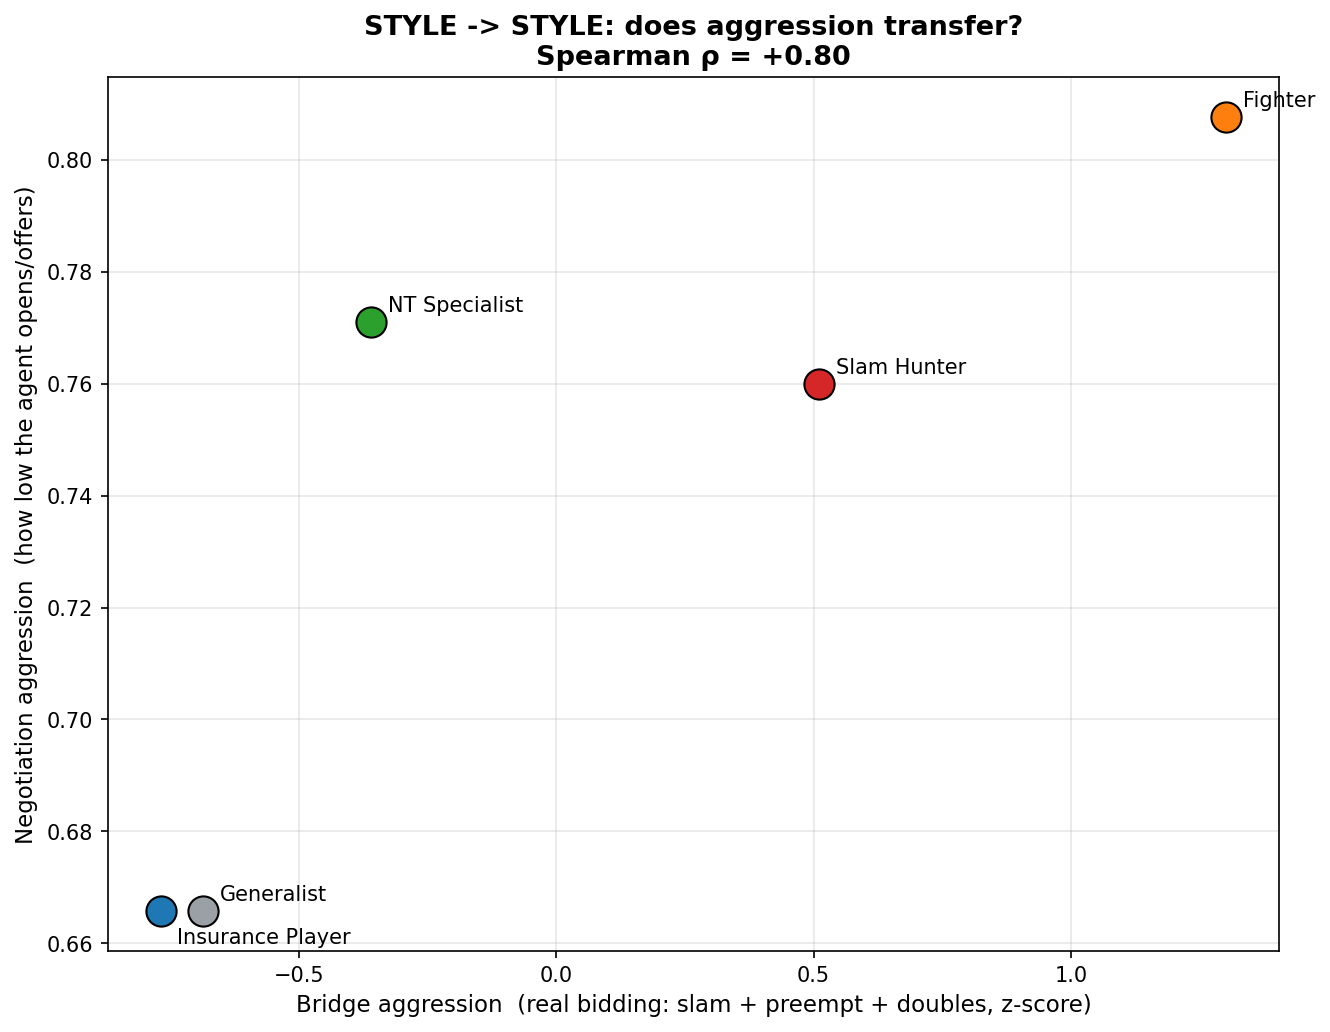
\includegraphics[width=0.78\textwidth]{../docs/images/style_alignment.png}
\caption{Cross-domain behavioural consistency: bridge aggression (real bidding)
vs.\ negotiation aggression (demand depth, how low the agent opens),
$\rho = +0.80$.}
\end{figure}

\section{The identity-disentangled crossover control (robustness to label bias)}
To rule out ``the agent is aggressive because we labelled it aggressive,''
each profile kept its identity but received the \emph{opposite} profile's
bridge skills (the identity-disentangled crossover control of
Chapter~\ref{ch:formal}). The correlation flipped from $+0.80$ to
$\mathbf{-0.90}$ ($p = 0.037$) - behaviour follows the injected bridge-derived
skills, not the label:

\begin{figure}[H]
\centering
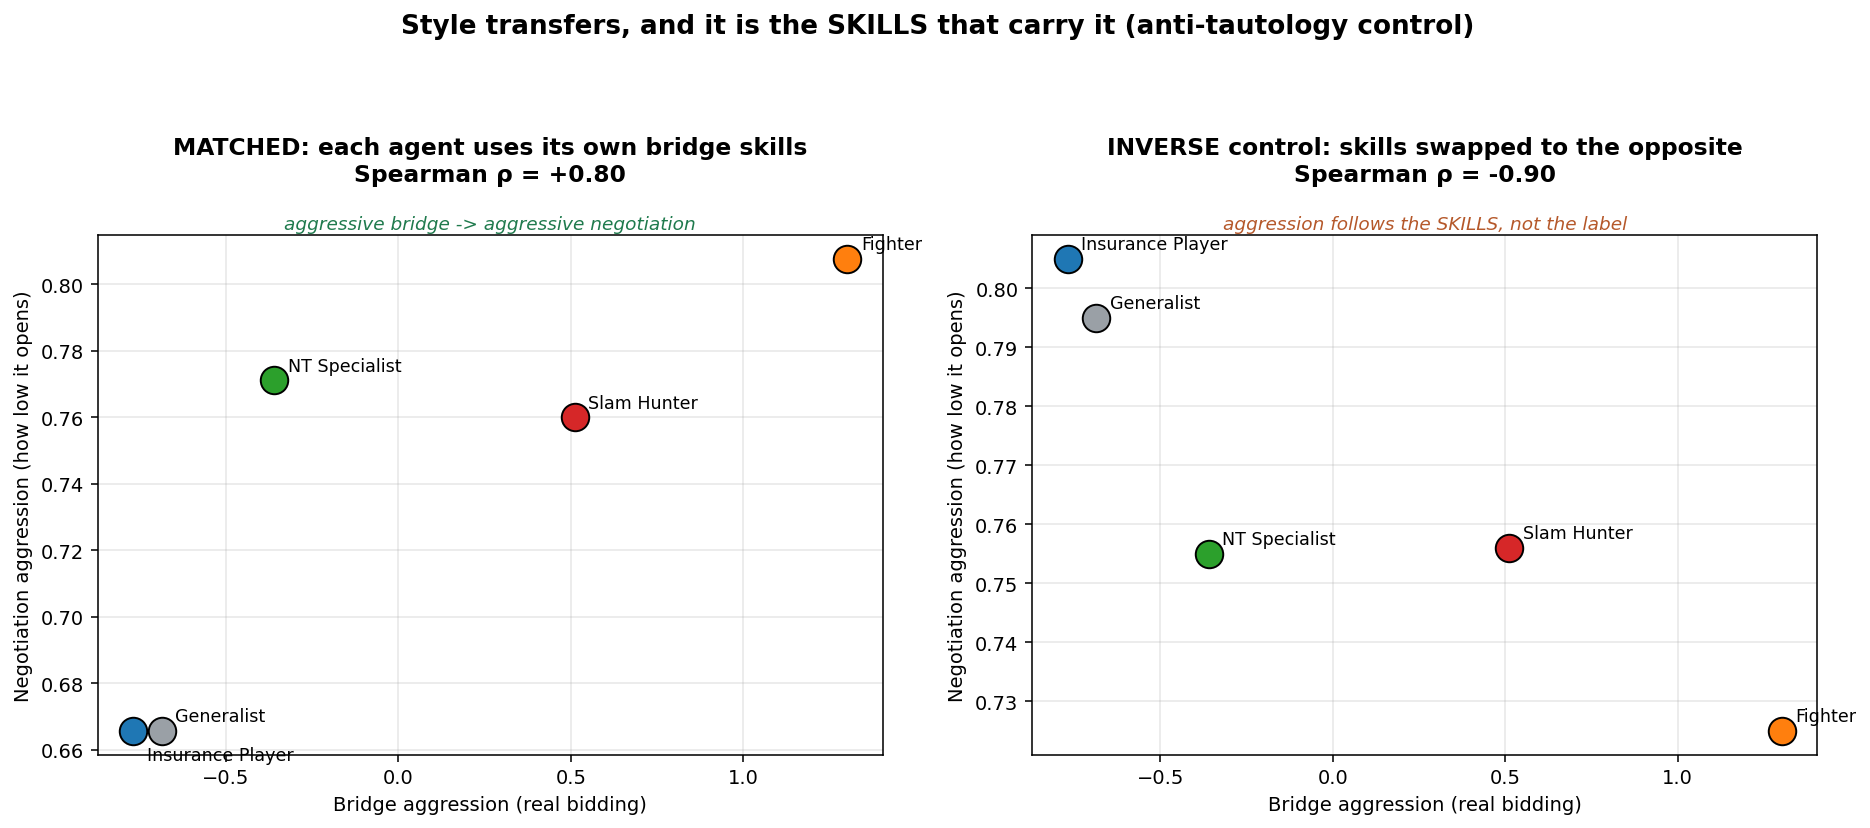
\includegraphics[width=\textwidth]{../docs/images/style_transfer_control.png}
\caption{Matched skills (left, $+0.80$) vs.\ swapped skills (right, $-0.90$):
the bridge-derived skills carry the disposition.}
\end{figure}

\section{Honest limitations}
With $n = 5$ profiles the consistency correlation is indicative
($p \approx 0.10$), not significant; negotiation is simulated (calibrated on
real human negotiations, but no same-person negotiation data exists); and the
Slam Hunter profile, defined by \emph{bidding} slams, may partly proxy
overall playing strength. These are documented, not hidden.

\chapter{The AI Layer: LLM Agents and Skill Engineering}
\label{ch:ai}

\section{Agent architecture}
All agents inherit from an abstract \texttt{BaseAgent} that owns the profile
signature, the LLM client, and a single decision choke-point. No agent calls
a provider SDK directly - every decision flows through one method, which
centralises retries, JSON parsing, temperature policy, and cost logging:

\begin{lstlisting}
class BaseAgent(ABC):
    def _decide(self, user_prompt, response_schema, purpose) -> dict:
        """The ONLY path to the LLM: schema-enforced, logged, retried."""
        response = self.client.generate(
            system=self.system_prompt, user=user_prompt,
            purpose=purpose, temperature=self.temperature,
            response_schema=response_schema)
        return response.json or json.loads(response.text)
\end{lstlisting}

Two concrete agents implement the domains: \texttt{BridgeAgent.make\_bid()}
(temperature $0$ for reproducibility; every returned call is validated by a
local, non-LLM legality checker and falls back to \texttt{Pass} if illegal)
and \texttt{NegotiationAgent.respond\_to\_offer()} (temperature $0.7$;
returns one of three actions, \texttt{counter}/\texttt{accept}/\texttt{walk\_away},
together with a counter-price).

\section{Clamping as a bounded-rationality constraint}
Because the LLM occasionally proposes a number outside the deal's plausible
band, that price is \emph{clamped} to the scenario's legal range -- forced to
lie between the seller's floor and its opening ask. This is best read not as a
``code workaround'' but as a formal \textbf{bounded-rationality} constraint in
the sense of Simon \cite{simon1955}: the environment imposes feasibility
limits on an otherwise free-form agent, preventing nonsensical pricing and
ensuring that a malformed reply cannot corrupt the downstream aggressiveness
measurement. The clamp affects only out-of-range outliers; it does not alter
the relative ordering of the profiles that the analysis depends on.

\section{Skill extraction and the identity-disentangled rule}
Stage 2 turns raw hands into a \emph{skill profile}: hands are chunked
(20--30 per call), sent with a strict JSON schema
(\texttt{response\_mime\_type="application/json"}), and aggregated across
chunks. The cardinal engineering rule: agents are \textbf{never} given
personality adjectives. The Fighter's card says \emph{``doubles opponents at
6--8$\times$ the field rate''} - a fact extracted from its players' real
auctions - not \emph{``be aggressive.''} Any cross-domain behaviour must
therefore \emph{emerge} from bridge-derived skills. The identity-disentangled
crossover control (Chapter~\ref{ch:keyresults}) is the executable test of this
rule: swapping the skills swaps the behaviour ($\rho: +0.80 \rightarrow -0.90$).

\section{Prompt engineering as configuration}
Prompts are code-reviewed artefacts, not ad-hoc strings: a central library
(\texttt{shared/prompts.py}) builds every character card from the same
template - identity line, 5--7 extracted skills, domain rules, a strict
output schema, and a few-shot example. Temperature, schema, and provider are
parameters, so an experiment is a configuration change, not a rewrite.

\section{Engineering against non-determinism}
LLMs are non-deterministic even at temperature $0$ (parallel GPU execution).
The system therefore treats reproducibility at the \emph{sample} level:
every (profile, deal) is run three times with majority voting; every raw
response is persisted to JSONL before aggregation; and all analyses are
recomputable from the persisted artefacts without new API calls. Deals
themselves come from a seeded generator, so the entire experiment replays
bit-identically up to the LLM boundary.

\section{A domain-expert validation skill}
Because an LLM can produce fluent but bridge-illegal or statistically
implausible output, the project ships a dedicated
\texttt{BridgeValidator} skill (\texttt{src/shared/bridge\_validator.py},
also exposed as the \texttt{/bridge-expert} slash command). It acts as an
automated bridge expert that checks every reported game statistic against
the duplicate-bridge rulebook and against the project's empirical baselines
(slam ${\approx}5.5\%$, partscore ${\approx}57\%$, NT ${\approx}28\%$,
penalty double ${\approx}8.5\%$), and against Nezer's minimum sample size
($n \geq 50$ declared boards). Each claim is returned under a fixed
four-part schema (Legality $\rightarrow$ Probability $\rightarrow$ Expert
analysis $\rightarrow$ Verdict), so a profile assignment such as
``slam\_rate $=0.20$ over $20$ boards'' is automatically flagged as
small-sample and rejected. This turns expert bridge judgement into a
reusable, testable software component rather than a manual review step.

\section{Provider-neutral LLM client}
A single \texttt{LLMClient} wraps Gemini (default), Claude, and OpenAI behind
one interface (an Adapter pattern). It implements exponential-backoff
retries, a per-request 60-second HTTP timeout (a hung socket once stalled a
1{,}500-call batch - the timeout converts hangs into retryable failures),
and a JSONL cost log per call (provider, model, tokens, latency, USD).
The cost log records ${\approx}\$1.69$ across $4{,}644$ logged calls; actual
out-of-pocket spend during development, including pre-logging experiments and
retried runs, was ${\approx}30$ ILS (${\approx}\$8$).

\chapter{Software Engineering}
\label{ch:se}

\section{Architecture: a single SDK entry point}
The codebase follows a strict facade discipline: every public operation is
reachable through \texttt{src/sdk.py}, and no function lives only in a
notebook or script. Modules are organised by pipeline stage:

\begin{lstlisting}
src/
  sdk.py                  # facade: the single public contract
  stage1_clustering/      # features, profiling, validation
  stage2_skills/          # chunker, extractor, aggregator
  stage3_agents/          # BaseAgent, BridgeAgent, NegotiationAgent
  stage4_simulate/        # bridge_game, bridge_auction, negotiation,
                          # monkey_agent (ZI-C), alignment
  features/double_dummy.py  # DDS perfect-play evaluator (endplay)
  shared/                 # llm_client, prompts, data_loader, logger
\end{lstlisting}

Design patterns in active use: \textbf{Facade} (\texttt{sdk.py}),
\textbf{Template Method} (\texttt{BaseAgent.\_decide()}),
\textbf{Adapter} (provider-neutral \texttt{LLMClient}),
and \textbf{Strategy} (interchangeable profile agents, including the
zero-intelligence \texttt{MonkeyAgent} baseline, which is duck-typed to drop
into every runner unchanged).

\section{Testing}
The project ships $100{+}$ \texttt{pytest} tests: pure-logic units (deal
generation, scoring, auction legality - 28 tests for the bridge engine
alone), the zero-intelligence baseline agent (legality of every random call,
reproducibility under a fixed seed), the double-dummy evaluator (known
fixtures: a 12-trick deal must score $6$NT${}=1.0$ and $7$NT${}=0.0$), and
the LLM-dependent layers tested by \emph{injecting a mocked client} - no
network, no API key, no cost:

\begin{lstlisting}
def test_monkey_bids_are_always_legal_over_many_auctions():
    monkey = MonkeyAgent(seed=1)
    for auction in AUCTION_FIXTURES:
        for _ in range(50):
            out = monkey.make_bid(HAND, auction)
            assert is_legal_call(out["bid"], auction)
\end{lstlisting}

\section{Reliability engineering}
The long simulation runs are engineered to survive real-world failure modes
observed during the project: a per-request HTTP timeout (hangs
$\rightarrow$ retries), per-board \emph{atomic} retry with pauses (rides out
provider 503 load spikes without losing the batch), and incremental JSONL
checkpointing with \texttt{flush()} after every board - a killed run keeps
all completed work and progress is observable from the file system.

\section{Reproducibility and data discipline}
Fixed seeds (\texttt{random\_state=42}) across scikit-learn and the deal
generator; raw data immutable (\texttt{data/raw} is read-only by
convention); every derived number traceable to a persisted artefact; and the
full history in Git under conventional-commit discipline
(\texttt{feat(stage4): ...}, \texttt{docs(guide): ...}). Every figure in
this portfolio is generated by a committed script - nothing is hand-drawn,
so documentation cannot drift from the data.

\section{Code quality and cost as an engineering budget}
Style and typing are enforced with \texttt{ruff}, type hints, and
Google-style docstrings on all public functions. LLM cost is treated as an
engineering budget: model selection is empirical
(\texttt{gemini-2.5-flash-lite} proved $10\times$ faster than the default
for this workload), and every call is metered. The logged production calls
cost ${\approx}\$1.69$; counting development iterations and retried runs, the
actual spend was ${\approx}30$ ILS (${\approx}\$8$), still well under the
\$50 cap.

\chapter{Conclusions and Future Work}

\textbf{Conclusions.} (1)~Elite bridge players form a behavioural continuum,
not clusters; statistically validated archetypes live in its extreme tails.
(2)~A skill metric that a zero-intelligence agent can beat is broken - the
ZI-C baseline test clearly changed this project's measurements.
(3)~Decision \emph{style} transfers across domains as cross-domain behavioural
consistency ($\rho = +0.80$, non-tautological by an executed
identity-disentangled crossover control); \emph{winning} does not transfer
cleanly, because winning is a property of the (style~$\times$~environment) pair.

\textbf{Future work.} More archetypes (finer partitioning of the 563 players)
for statistical power; multi-dimensional negotiation-style measurement
(concession speed, walk-away propensity); cross-model replication
(Claude/GPT); separating style from playing strength; and ultimately real
same-person negotiation data.

\section*{Path to an article-based dissertation}
\addcontentsline{toc}{section}{Path to an article-based dissertation}
Under LUT University's regulations a doctoral dissertation may be article-based,
comprising several peer-reviewed papers plus an introductory summary. NegoPlay
is positioned as the empirical baseline (Paper~I) of such a dissertation, with
two planned extensions that build directly on the existing SDK:

\begin{itemize}[leftmargin=*]
  \item \textbf{Paper~I (this study).} Empirical proof of concept for
        cross-domain behavioural consistency via bridge profiles and
        LLM-based negotiation agents.
  \item \textbf{Paper~II (algorithmic extension).} Replace hand-engineered
        features in Stage~1 with learned hand representations
        (BridgeHand2Vec \cite{sztyber2023}, a DDS-grounded embedding of the
        13-card hand) to sharpen the archetypal boundary profiling.
  \item \textbf{Paper~III (cross-platform human validation).} Calibrate the
        NegoPlay simulators against real human negotiation data and run live
        human-subject studies to validate the predictive accuracy of the
        profiled agents.
\end{itemize}

% =====================================================================
% REFERENCES (for Part I — the Final Summary Report)
% =====================================================================
\clearpage
% Let thebibliography emit its own chapter heading (report class does this
% automatically); rename it to "References" and register it in the master TOC.
\renewcommand{\bibname}{References}
\begin{thebibliography}{9}
\addcontentsline{toc}{chapter}{References}

\bibitem{cutler1994}
Cutler, A., \& Breiman, L. (1994). Archetypal Analysis.
\emph{Technometrics}, 36(4), 338--347.

\bibitem{godesunder1993}
Gode, D.~K., \& Sunder, S. (1993). Allocative Efficiency of Markets with
Zero-Intelligence Traders: Market as a Partial Substitute for Individual
Rationality. \emph{Journal of Political Economy}, 101(1), 119--137.

\bibitem{he2018}
He, H., Chen, D., Balakrishnan, A., \& Liang, P. (2018). Decoupling Strategy
and Generation in Negotiation Dialogues. In \emph{Proceedings of EMNLP 2018}.

\bibitem{lockett2007}
Lockett, A.~J., Chen, C.~L., \& Miikkulainen, R. (2007). Evolving Explicit
Opponent Models in Game Playing. In \emph{Proceedings of the Genetic and
Evolutionary Computation Conference (GECCO 2007)}.

\bibitem{rong2019}
Rong, J., Qin, T., \& An, B. (2019). Competitive Bridge Bidding with Deep
Neural Networks. In \emph{Proceedings of AAMAS 2019}.

\bibitem{silver2017}
Silver, D., et al. (2017). Mastering the Game of Go without Human Knowledge.
\emph{Nature}, 550, 354--359.

\bibitem{simon1955}
Simon, H.~A. (1955). A Behavioral Model of Rational Choice.
\emph{The Quarterly Journal of Economics}, 69(1), 99--118.

\bibitem{sztyber2023}
Sztyber-Betley, A., Ko{\l}odziej, F., Betley, J., \& Duszak, P. (2023).
BridgeHand2Vec: Bridge Hand Representation. In \emph{Proceedings of ECAI 2023}
(FAIA, vol.~372). arXiv:2310.06624.

\bibitem{talwadker2022}
Talwadker, R., et al. (2022). CognitionNet: A Collaborative Neural Network for
Play Style Discovery in Online Skill Gaming Platform. In \emph{Proceedings of
KDD 2022}.

\bibitem{tennant2025}
Tennant, E., Hailes, S., \& Musolesi, M. (2025). Moral Alignment for LLM
Agents. In \emph{Proceedings of ICLR 2025}.

\end{thebibliography}

% =====================================================================
% PART II — PREPARATORY REPORT (full, included)
% =====================================================================
\part{Preparatory Report}
% The bundled sub-reports keep their own internal "Chapter 1, 2, ..." numbering
% on their pages, so we list them in the master TOC by TITLE ONLY (no master
% chapter number) to avoid a mismatch. Emptying \thechapter makes pdfpages'
% \numberline render blank; the page links and bookmarks are unaffected.
\renewcommand{\thechapter}{}%
% Chapters are registered into the single master TOC below (page numbers are
% physical pages within main.pdf, taken from main.toc; pdfpages adds the offset).
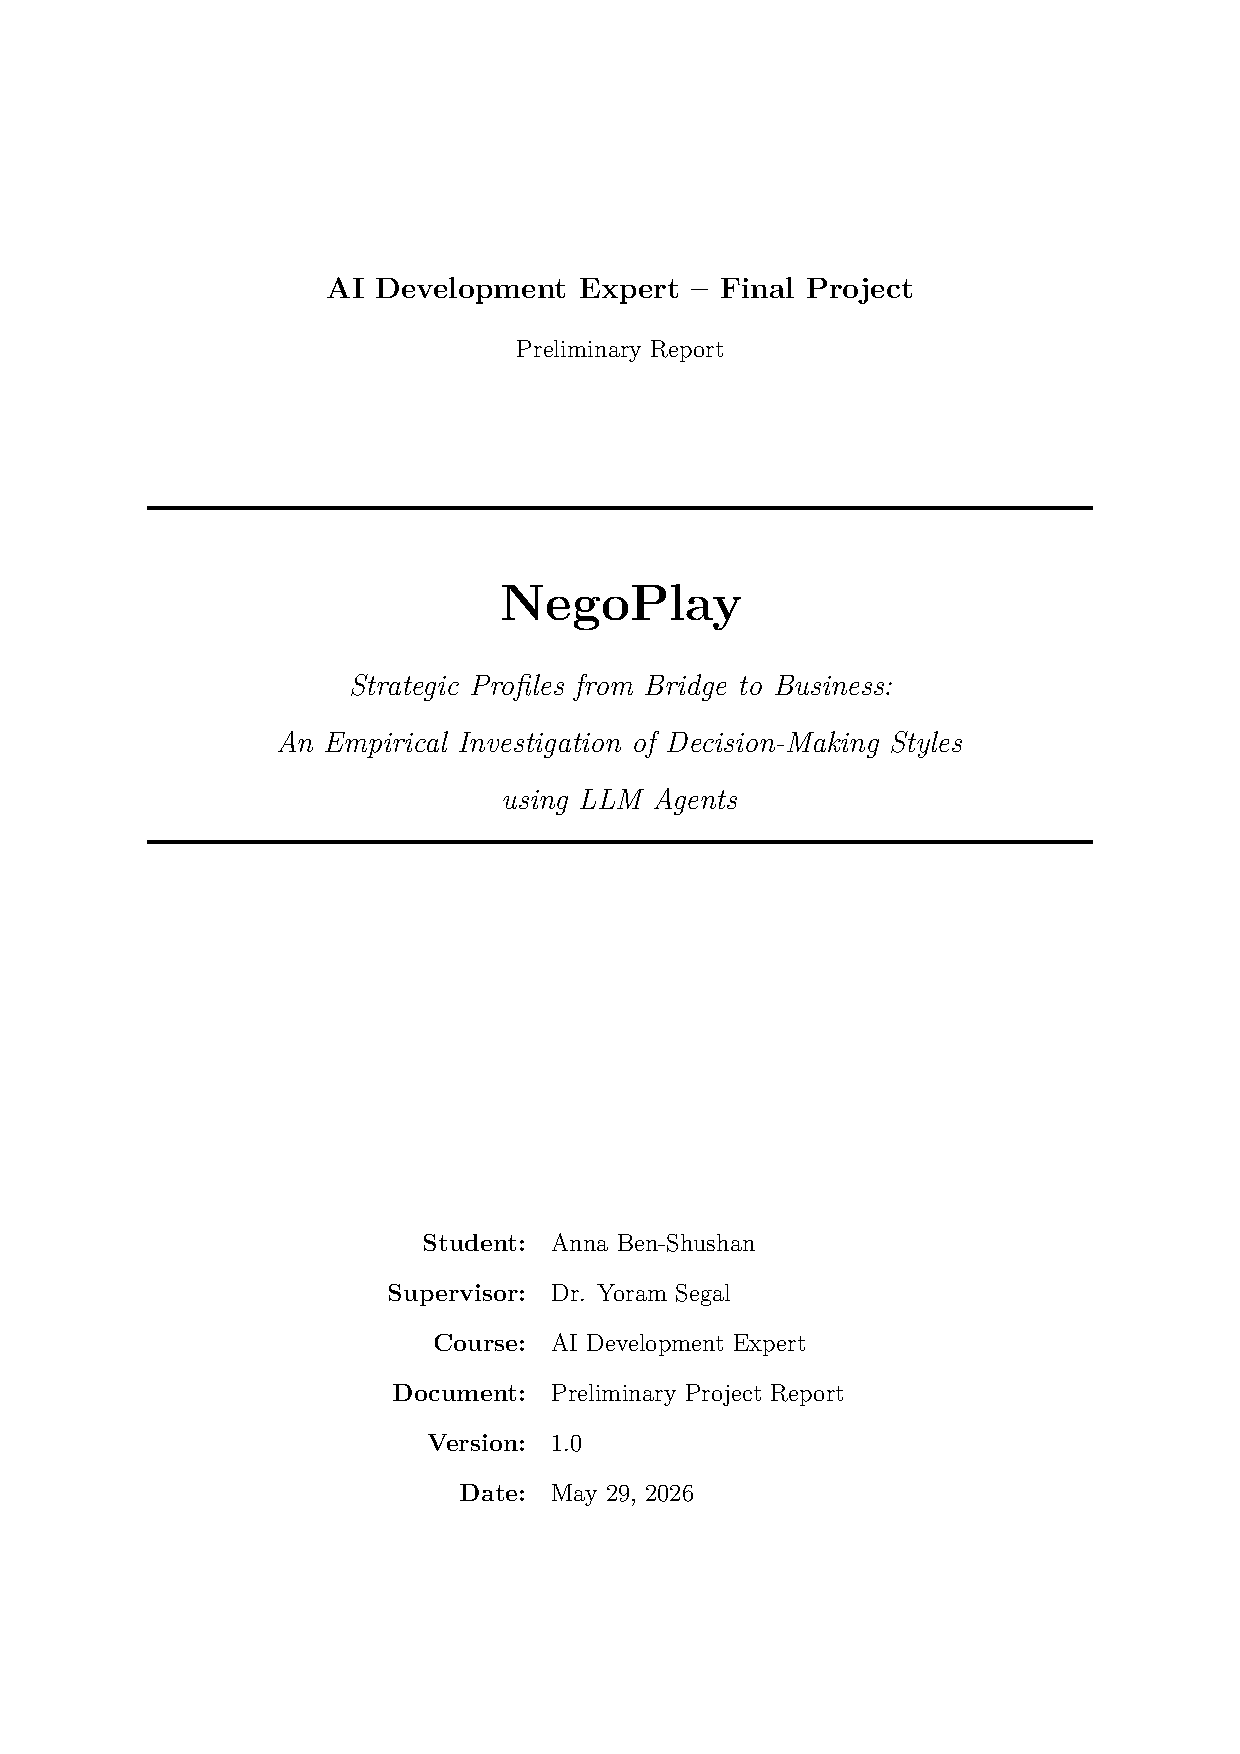
\includepdf[pages=-, addtotoc={%
  1,chapter,1,{Introduction},pr1,%
  4,chapter,1,{Research Question and Objectives},pr2,%
  5,chapter,1,{Methodology},pr3,%
  14,chapter,1,{Technical Architecture and Mathematical Foundations},pr4,%
  23,chapter,1,{Results: Stage 4 Cross-Domain Alignment},pr5,%
  28,chapter,1,{Work Packages},pr6,%
  30,chapter,1,{Deliverables and Success Criteria},pr7,%
  32,chapter,1,{Risk Management},pr8,%
  35,chapter,1,{Summary},pr9,%
  36,chapter,1,{Reproducibility Package (Appendix)},pr10%
}]{main.pdf}

% =====================================================================
% PART III — BUSINESS PLAN (full, included)
% =====================================================================
\part{Business Plan}
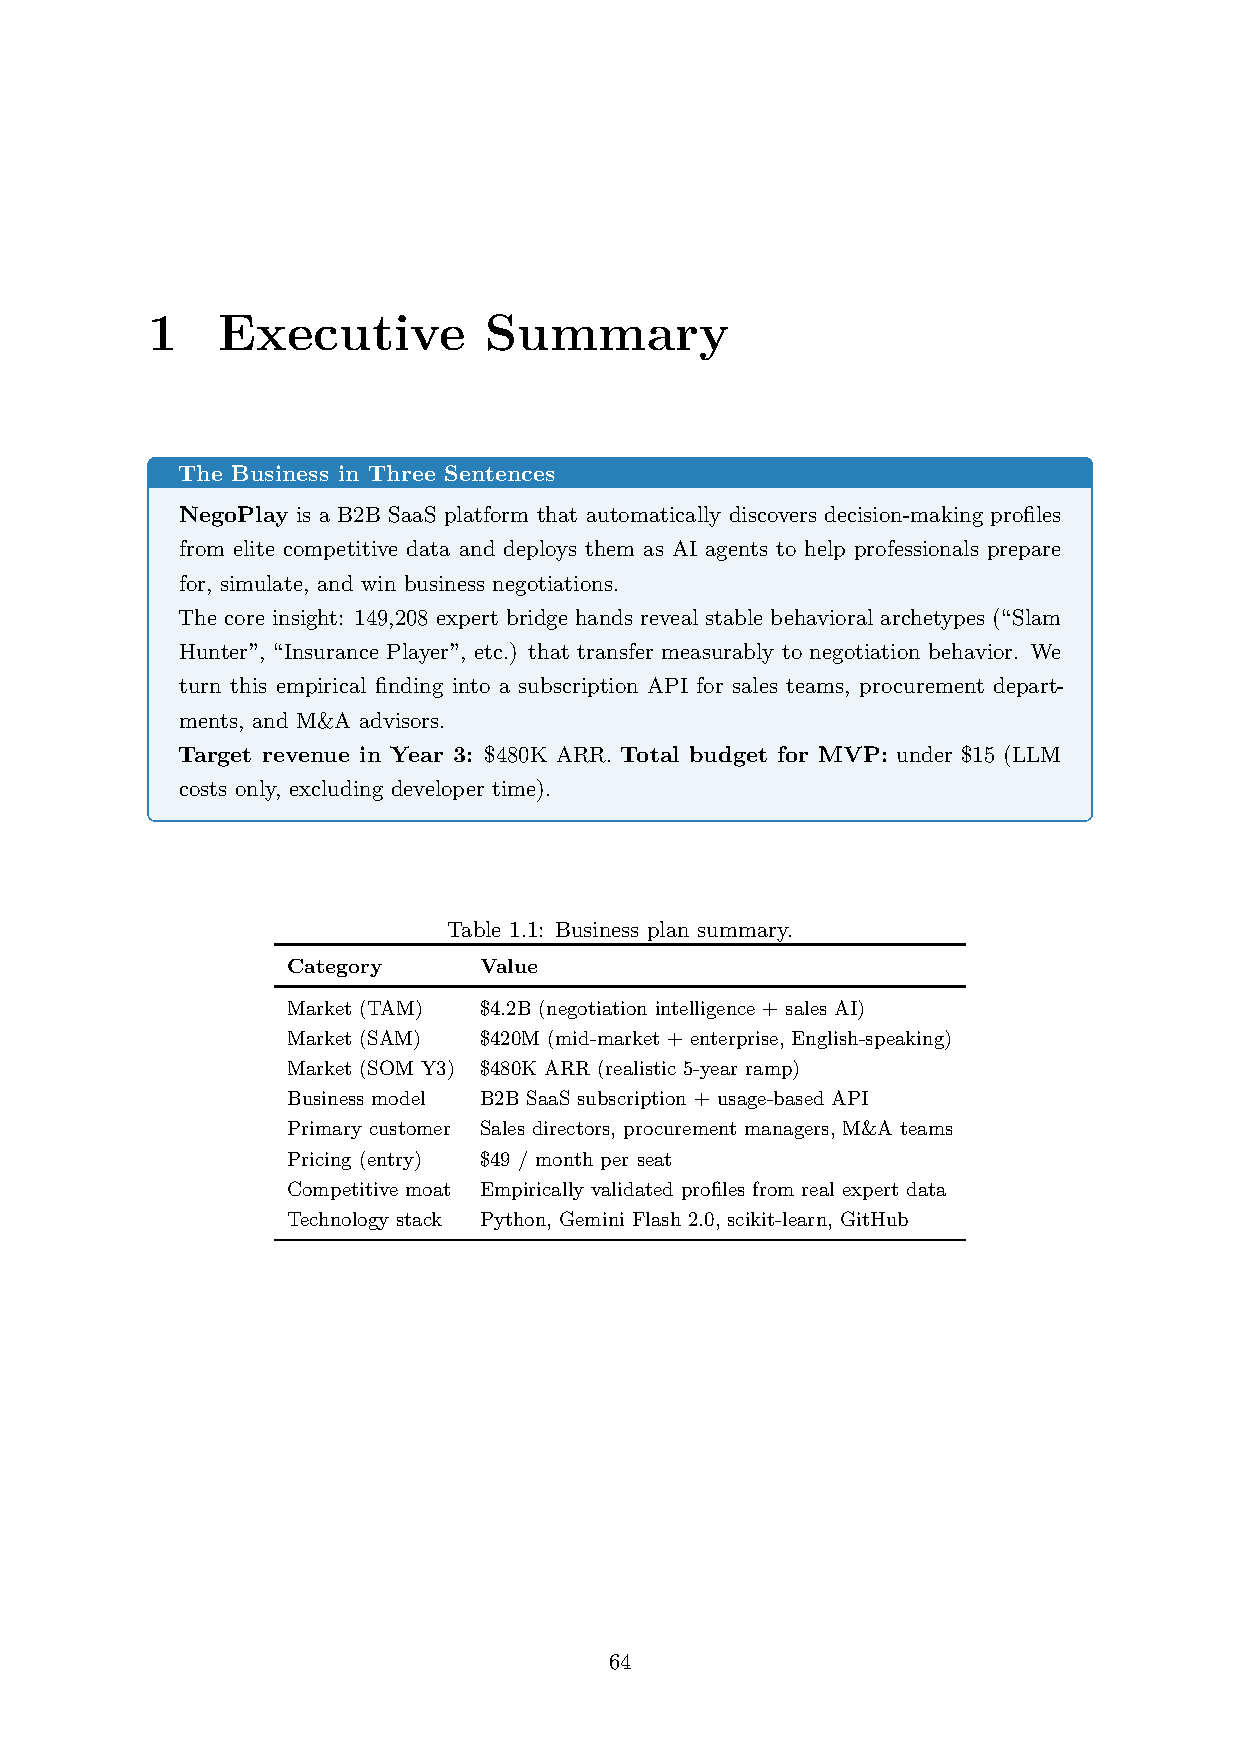
\includepdf[pages=-, addtotoc={%
  1,chapter,1,{Executive Summary},bp1,%
  2,chapter,1,{The Problem},bp2,%
  3,chapter,1,{The Solution},bp3,%
  5,chapter,1,{Market Analysis},bp4,%
  7,chapter,1,{Business Model and Pricing},bp5,%
  10,chapter,1,{Competitive Landscape},bp6,%
  11,chapter,1,{Go-to-Market Strategy},bp7,%
  13,chapter,1,{Roadmap and Milestones},bp8,%
  14,chapter,1,{Financial Projections},bp9,%
  15,chapter,1,{Business Risks},bp10,%
  16,chapter,1,{Team},bp11,%
  17,chapter,1,{Conclusion},bp12%
}]{business_plan.pdf}

\end{document}
